\documentclass{article}
\usepackage[utf8]{inputenc}
\usepackage[left=2.5cm,right=2.5cm,top=2.5cm,bottom=2.5cm]{geometry}

\usepackage{notes2bib}
\usepackage{amsmath}
\usepackage{amssymb}
\usepackage{hyperref}
\usepackage{graphicx}

\usepackage{epstopdf}
\usepackage{epsfig}

\usepackage{paralist} % inline list

\usepackage{amsthm} % theorem and definition
\newtheorem{mydef}{Definition}
\newtheorem{exmp}{Example}

\usepackage{tikz}
\usepackage{xytree}

\usepackage{color}

\usepackage{hhline}
\usepackage{float}
\restylefloat{table}

\title{High-level image interpretation using logical and morphological approaches}
\author{Yifan YANG}

\begin{document}

\maketitle
\section{Introduction}
 High-level semantics extraction from an image is an interesting research area for automatic image understanding in artificial intelligence.
 Many related fields like image annotation, activity recognition and  decision-support systems take advantage of semantic content.
 As advanced as AI has become, it still remains a big challenge for computers to accomplish complex understanding tasks as humans do.
 %However, computers still have difficulties to accomplish complex understanding as humans.  
 Digital image itself is a numerical representation which does not represent explicitly semantic information. 
 Moreover, beyond a single object understanding based on low level features such as colors and forms, we focus on a complex description which relies on context information like spatial relations
 between diverse objects as well as prior knowledge on the application domain.
 For instance, in the context of medical applications, the understanding task can be formulated as giving an abstract description of a pathological brain volume, such as in Figure~\ref{fig:patho_brain}. 
  According to different levels of anatomical prior knowledge on brain pathology, two possible descriptions could be given:
 \begin{itemize}
  \item an abnormal structure is present in the brain,
  \item a peripheral non-enhanced tumor is present in the right hemisphere.
 \end{itemize}
%  according to different prior knowledge of anatomic pathology of the  brain.
%  The second explanation can only be inferred by an experienced doctor with background knowledge.
 In this thesis, a high-level interpretation is regarded as an explanation of what we have seen in the image.
 This process is an inference based on  prior knowledge to link the abstract description and the observed context of the scene.
  \begin{figure}[h]
  \centering
   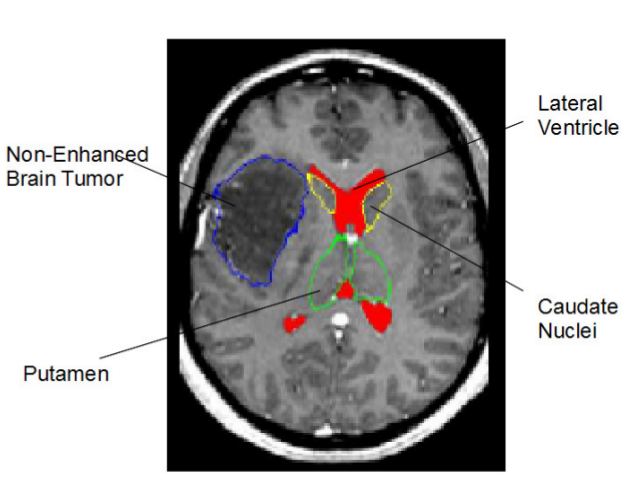
\includegraphics[scale=.2]{./figures/patho_brain.png}
   \caption{\label{fig:patho_brain} A slice of a pathological brain volume (MRI acquisition), where some structures are annotated.}
 \end{figure} 
\subsection{Problem formulation}
According to the objective pointed out in the previous part, the aim is to extract high-level semantic information from a given image and translate it at a linguistic level.
Concretely, we are interested in the interpretation of cerebral images with tumors. The high-level information corresponds to the presence of diverse types of pathologies
 as well as descriptions of brain structures and spatial relations among them in a brain image. 
%  To deal with this problem, prior knowledge at a linguistic level helps the decision making procedure since the semantics is not included in the image.
 In the context of this thesis, the decision process is modeled as an abductive reasoning~\cite{aliseda1997seeking} using a logical formalism, 
 which is an inference mechanism from facts to explanations.
The objective of this thesis is to build a generic logic based formalism as well as  to develop an appropriate reasoning process for image interpretation, 
 allowing us to extract a set of suitable candidates as potential hypotheses for a given image and to select the ``best'' one by a defined criterion.  
%  The knowledge representation is based on an ontology.
 In image interpretation, spatial relationships are important when objects of similar appearance are present in the image, especially in magnetic resonance imaging (MRI).
 Such relationships have then to be included in the representation and in the reasoning process.
  
% In this thesis, a description may not include in the knowledge base and we need to construct it 
% Formal language is a good choice with solid math representation
% First talk about what we need to resolve in this field, which problem, orientations we will take
% Write a general schema here and for each part, what do we have 
  \begin{figure}[h]
  \centering
   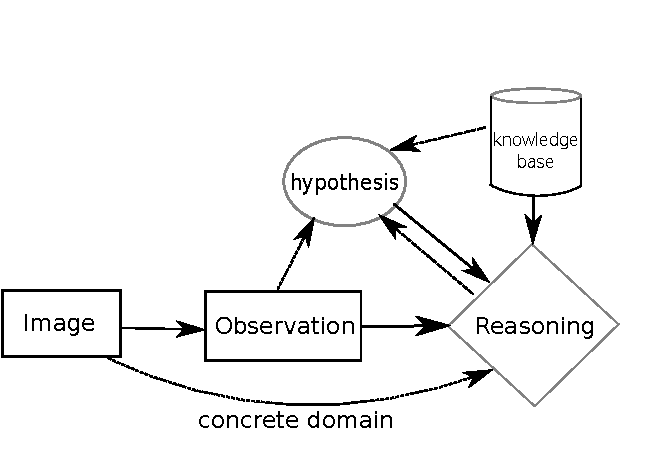
\includegraphics[scale=.8]{./figures/intro_schema.pdf}
   \caption{\label{fig:intro_schema} A general schema of image interpretation task in the thesis.}
 \end{figure} 
Figure~\ref{fig:intro_schema} shows the major components of our framework in this thesis. The given image is translated into symbolic representations in terms of logical form at the beginning.
The image can also serve as the concrete domain in both the knowledge base and the reasoning process. 
Concrete domain is used as a real model to represent abstract terminologies in image space.
A hypothesis of an description might be generated from the observation or the axioms in the knowledge base.
The relations between the hypothesis and reasoning are two directions, which allows validating the hypothesis with the help of standard reasoning and
building a possible hypothesis within non-standard reasoning processes.

To summarize the ongoing and future work, we need to answer the following questions:
\begin{itemize}
 \item \textit{How to model knowledge and formalize an appropriate representation in a given application domain? (Section~\ref{sec:pre})}
 \item \textit{How to connect image level representation and symbolic level representation? (Section~\ref{sec:qsr})}
 \item \textit{How to overcome the semantic gap between numerical representation and qualitative representation of spatial relationships? (Section~\ref{sec:qsr})}
 \item \textit{How to generate hypotheses to explain the observed scene? (Section~\ref{sec:abd} and Section~\ref{sec:persp})}
 \item \textit{How to define a criterion to choose a ``best'' explanation in our case? (Section~\ref{sec:abd} and Section~\ref{sec:persp})}
\end{itemize}
 %  The semantic gap is still an open problem in the field of image interpretation. 
%  This is due to the different level between the numerical measurement in the image and qualitative representation in an expert knowledge.

 \subsection{Related work}
Recognition of perceptual objects and scene understanding, which translate low level signal information into meaningful semantic information, belong to one of the fundamental abilities of human beings.
Semantics is important in image analysis, for various tasks such as image annotation, event detection and diagnostic problems.
In some specific domains, like medical imaging and remote sensing, image interpretation combines image processing with artificial intelligence techniques to derive reasonable semantics.  
Prior knowledge is intensively used by experts who interpret visually an image. Evidently it should then also be used by machines to associate semantics with the image.  
However, image interpretation still faces some difficulties, one of which is how to accurately associate perceptual data with appropriate concepts. Without an expert knowledge,
such a link cannot be established. This relation between visual perception and high-level linguistic expression is called \textit{semantic gap}.


As a high level process of exploiting semantic in the scene, image interpretation involves two levels:
\begin{itemize}
 \item relating low level features to semantics (from pixels to semantic information)~\cite{Bloch2005fuzzy,fouquier2012sequential,Hudelot2008fuzzy,nempont2013constraint}.
 \item inferring the description from the semantic image content (from semantics to explanation)~\cite{atif2014explanatory,Espinosa07multimedia}.
\end{itemize}

Roughly speaking, the first level describes what is happening while the second one describes how it is happening~\cite{tsotsos1992image}.
The first level has been mainly studied in the field of multiple objects recognition. 
Image interpretation maps regions or groups of regions onto labels corresponding to semantic concepts (e.g. labels of anatomical structures for medical images).
Various approaches employ Bayesian networks with a combination of semantics and probabilistic inference mechanisms~\cite{Luo2005Bayesian,Niko2009evidence,Singhal2003proba}.
These techniques provide inference mechanisms by attempting to construct co-occurrence objects and contextual information with a probabilistic model for reasoning.

Further, a hierarchical representation of knowledge base is proposed, called image grammar~\cite{tu2014joint,zhu2006stochastic}. The grammar is a structured knowledge represented by an And-Or graph.
In this graph, a global description of a scene is decomposed into parts, objects until primitive pixel patches from top to bottom.
An And-node consists of a set of successive components and an Or-node is composed by alternative nodes.
A parsing method is proposed as inference within a probabilistic model in each node~\cite{han2009bottom,wu2011numerical}. 

The second level consists in reasoning at the language (knowledge) level.
For the purpose of giving an adequate explanation, the second level is a logic-based reasoning to depict the image with a deep and abstract description from the point of view of an expert.
There is not much work on image interpretation using logical knowledge representation and reasoning. 
However, formal language based on logic formalism has  strong associated semantics for knowledge representation as well as reasoning processes. 
An aggregation concept is proposed in~\cite{Espinosa07multimedia} to represent a complex event or scene concerning occurrence objects, as well as spatial and temporal constraints configuration.
According to these defined aggregation and specific rules, a high-level interpretation is able to be inferred~\cite{neumann2008scene}.
In addition, the results using Bayesian networks and image grammars are limited to defined descriptions.
A complex description can also be generated when non-explicitly presented in the knowledge base~\cite{atif2014explanatory}.

% Because the Bayesian network and image grammar method are  

%  Since a large number use of multimedia in daily life, semantic information extraction of images has been variously studied in many fields such as image annotation, event detection and diagnostic problems.
%  These areas involve different methodologies like machine learning . Many work 
% Image interpretation based on knowledge representation


% What knowledge is needed for image interpretation?
% How to represent it?
% Formal language
% How to produce an inference to get the result?
% 
%  We need to interpret it with prior knowledge.
%  In this thesis, we focuses on diagnostic problem (decision support system) in LOGIMA project
%  The knowledge may not be accurate presented and correspond what we are looking at. Lack of expressivity graph representations.
% 
% The context and  main objective of my thesis will be developed in this part.
% I would like to present a short bibliography of image interpretation. Then, I would like to present
% that we focus on diagnostic problem and we treat this problem as an abductive reasoning with a knowledge base represented by description logics.
% I also explain the reason why we choose this kind of method (its advantages).

\section{Preliminaries}\label{sec:pre}
\subsection{Ontology}
Experts' knowledge is expressed in terms of diverse vocabulary of special domain in natural language which is difficult to be interpreted by machines.
In order to facilitate automated reasoning process with background knowledge base, a structural semantic based model is  an effective means to represent the prior knowledge.
The term ontology is derived from philosophy and then used for the purpose of expressing common sense knowledge in computer science~\cite{alexander1986knowledge}.
Since then, ontologies was adopted for image interpretation tasks~\cite{bannour2011towards,Hudelot2008fuzzy,town2006ontological}.
Ontologies are defined as “\textit{a formal specification of a shared conceptualization}"~\cite{studer1998knowledge},
which deal with modeling a universal and reusable knowledge among different applications for a specific domain.
Ontologies is also studied for reasoning service within its expressive formal description. 
An ontology mainly contains  \textit{individuals}, \textit{concepts}, \textit{properties} and \textit{axiom rules}. 
These components enable the background knowledge to be understood and processable by machines.

\subsection{Description Logics}
As mentioned above, ontologies require a formal representation language and well-defined semantics for reasoning services. 
Description Logics (DLs) is a family of knowledge representation logical formalisms, which is seen as good candidates for ontologies~\cite{horrocks1999description}.
The basic elements of Description logics are concepts (unary predicates), roles (binary predicates) and individuals.
Besides the formal knowledge representation, the other reason of treating DLs as an important logical formalism is its ability of reasoning process.
Implicit information can be inferred from explicit knowledge description, such as satisfiability checking~\cite{baader2003description}. 
In this part, we introduce syntax and semantics of a description logic language $\mathcal{ALC}$ as well as its reasoning services.
\subsubsection{Syntax and semantics}
We first recall the syntax and semantics of the basic language of Description Logics ($\mathcal{ALC}$).
\begin{mydef}[Signature]
 The syntax of a Description Logic is defined over a signature, which is defined as three disjoint sets $Sig~=~(N_C,~N_R,~N_I)$. $N_C$ is a set of concept names that refers to a set of entities
 with the same characteristics. $N_I$ is a set of individuals that contains instances of the concepts in $N_C$.  $N_R$ is a set of role names that refers to the binary relationships between 
 two individuals or two concepts.
\end{mydef}


\begin{mydef}[Concept expression]
 The set of concept expression is recursively built from the signature such that:
 \begin{itemize}
  \item all the concept names, as well as $\top$ (top concept) and $\bot$ (bottom concept) are concepts,
  \item if $C$ and $D$ are two concepts in $N_C$ and $r$ is a role in $N_R$
  then $\neg C$ (negation), $ C\sqcap D$ (conjunction), $ C\sqcup D$ (union), $ \exists r.C$ (existential quantification), $\forall r.C$ (universal quantification) are also concepts.
 \end{itemize}
 Let $\mathfrak{C}$ be the infinite set of all the concepts that can be defined using constructors and signature elements.
\end{mydef}


\begin{mydef}[Terminological box (TBox) and assertional box (ABox)]
A general concept inclusion axiom (GCI) is an expression of the form $C\sqsubseteq D$ for two  concepts. 
An equality is an expression of the form $C\equiv D$. An equality can be written in terms of GCI: $C\sqsubseteq D$ and $D\sqsubseteq C$.
A TBox is a finite set of GCIs (an equality is expressed by two GCIs), denoted by $\mathcal{T}$.

An ABox is a set of individual assertions: $a:C$, $b:D$ and $(a,b):r$, where $a\in N_I$ and $b\in N_I$ are two instances of concepts $C$ and $D$, called concept assertions, and
the binary relation between $a$ and $b$ is an assertion of role $r$, called role assertion. An ABox is denoted by $\mathcal{A}$.

A knowledge base is a pair of TBox and ABox: $\mathcal{K}=(\mathcal{T},\mathcal{A})$.
\end{mydef}



\begin{mydef}[Model of $\mathcal{ALC}$]
An interpretation $\mathcal{I}=(\Delta^\mathcal{I},\cdot^\mathcal{I})$ provides the semantics of concepts and roles. $\Delta^\mathcal{I}$ is a non-empty set which indicates the entire
``world" of the application domain. $\cdot^\mathcal{I}$ is an interpretation function which connects concept and individual symbols to $\Delta^\mathcal{I}$ and roles to $\Delta^\mathcal{I} \times \Delta^\mathcal{I}$.
\begin{itemize}
 \item Every concept $C\in N_C$ is interpreted as a subset of $\Delta^\mathcal{I}$, represented by $C^\mathcal{I}\subseteq \Delta^\mathcal{I}$.
 \item Every  role $r$ is interpreted as a subset of $\Delta^\mathcal{I}\times\Delta^\mathcal{I}$, denoted as $r^\mathcal{I}\subseteq \Delta^\mathcal{I}\times\Delta^\mathcal{I}$.
 \item Every individual $a \in N_I$ is interpreted as an element in the set $\Delta^\mathcal{I}$, denoted as $a^\mathcal{I} \in \Delta^\mathcal{I}$.
\end{itemize}
The interpretation for concept expressions and axioms in the knowledge base are shown in Table~\ref{tab:interpretation}.
\end{mydef}
 \begin{center}
 \begin{table}[H]
 \begin{tabular}{|c|c|c|c|}
	\hline
	Constructor & Syntax & Semantics & Example\\
	\hline
	Atomic Concept & $C$ & $ C^{\mathcal{I}}\subseteq \Delta^{\mathcal{I}} $ & $Human$ \\ 
	Negation & $ \neg C$ & $\Delta^{\mathcal{I}}\backslash C^{\mathcal{I}}$ & $\neg Human$ \\ % Content row 1
	Top & $\top$ & $\top^{\mathcal{I}}=\Delta^{\mathcal{I}}$ & $All$ \\ % Content row 2
	Bottom & $\bot$ & $\bot^{\mathcal{I}}=\emptyset^{\mathcal{I}}$ & $Nothing$ \\
	Conjunction & $ (\mathit{C}\sqcap\mathit{D}) $ & $C^{\mathcal{I}}\cap D^{\mathcal{I}}$ & $Human\sqcap Male$ \\ % Content row 4
	Disjunction & $ (\mathit{C}\sqcup\mathit{D})$  & $C^{\mathcal{I}}\cup D^{\mathcal{I}}$ & $Female \sqcup Male$ \\ % Content row 5
	Universal Qualification & $ \forall R.\mathit{C}$ & $\{ x \in \Delta^{\mathcal{I}} \mid \forall y \in \Delta^{\mathcal{I}} :\langle x,y\rangle\in R^{\mathcal{I}} ~implies~ y \in C^{\mathcal{I}} \}$ & $\forall hasChild.Human$ \\ % Content row 6
	Existential Restriction  & $ \exists R.\mathit{C}$ &  $\{ x \in \Delta^{\mathcal{I}} \mid \exists y \in \Delta^{\mathcal{I}} :\langle x,y\rangle\in R^{\mathcal{I}} ~and~ y \in C^{\mathcal{I}} \}$ & $\exists hasChild.Female$ \\ % Content row 7
	\hline
	Subsumption & $C \sqsubseteq D$ & $C^{\mathcal{I}} \subseteq D^{\mathcal{I}}$ & $Man \sqsubseteq Human$ \\ 
	Concept definition & $C \equiv D$ & $C^{\mathcal{I}} = D^{\mathcal{I}}$ & $Father \equiv Man \sqcap \exists hasChild.Human$ \\ 
	Concept Assertion  & $a:C$ & $a^{\mathcal{I}} \in C^{\mathcal{I}}$ & $John:Man$\\ 
	Role Assertion & $(a,b):R$ & $\langle a^{\mathcal{I}},b^{\mathcal{I}}\rangle \in R^{\mathcal{I}}$ & $(John,Lea):hasChild$ \\
	\hline
	\end{tabular}
    \caption{Syntax and interpretations of $\mathcal{ALC}$.}
    \label{tab:interpretation}
\end{table}
\end{center} 

An example of the knowledge base referring brain anatomy is as follows\footnote{Due to the limited space, left and right lateral ventricles are abbreviated to LVl and LVr.
Similarly, left and right caudate nuclei are denoted by CNl and CNr}:
\begin{align*}
 TBox=\{ Hemisphere &\sqsubseteq \exists isPartOf. Brain\\
	 BrainStructure &\sqsubseteq \exists isPartOf. Brain\\
	 BrainDisease &\sqsubseteq \exists isPartOf. Brain \sqcap \neg BrainStructure\\
	 Tumor  &\sqsubseteq BrainDisease\\
	 LVl &\sqsubseteq BrainStructure \sqcap \exists (rightOf \sqcap closeTo). CNl\\
	 LVr &\sqsubseteq BrainStructure \sqcap \exists (leftOf \sqcap closeTo). CNr\\
	 CNl &\sqsubseteq BrainStructure\\
	 CNr &\sqsubseteq BrainStructure\\
\\
 ABox=\{ a&: CNl \\
	 b&: unknown object\\
	 c&: Brain \\
	 \langle a,b\rangle &: leftOf, closeTo \\
	 \langle b,c\rangle &: isPartOf\}
\end{align*}
This knowledge base  example demonstrates a practical way to represent brain anatomy. 
For instance, $LVl \sqsubseteq BrainStructure \sqcap \exists (rightOf \sqcap closeTo). CNl$ expresses that
the left lateral ventricle belongs to the brain structure which is on the right of and close to the left caudate nucleus.
In the ABox, $a,b,c$ are individuals of observed objects in the image. $a: CNl$ is a concept assertion and 
$\langle b,c\rangle : isPartOf$ is a role assertion, expressing that $b$ is a part of $c$.

\subsubsection{Reasoning services}
Implicit information which is not explicitly defined in the knowledge base needs to be inferred with reasoning services.
Reasoning services in Description Logic are decision procedures based on a knowledge base model. 
The basic reasoning on concept in Description Logics is subsumption checking (written as $\mathcal{T}\vDash C\sqsubseteq D$) and 
concept satisfiability checking (written as $\mathcal{T}\nvDash C\equiv \bot$).
Subsumption checking is a decision procedure to check whether a concept $D$ is more general than another concept $C$.
Checking satisfiability of a concept $C$ is a decision procedure to determine whether $C$ has a model with respect to the TBox.
Complex reasoning services are built based on the basic ones. For example, classification is a decision procedure  to find subconcept and superconcept 
relationships between concepts in a given terminology. This allows us to find a position in terminological hierarchy.
Therefore, classification can be reduced to subsumption checking of each pair of concepts in the given terminology.
The definitions of subsumption and satisfiability of a concept are introduced as follows \cite{baader2003description}:
\begin{itemize}
\item subsumption checking: $\mathcal{T}\vDash C\sqsubseteq D$ if $C^\mathcal{I}\subseteq D^\mathcal{I}$ for every model of $\mathcal{I}$ of $\mathcal{T}$.
\item concept satisfiability: $C$ is satisfiable with respect to $\mathcal{T}$ if there exists a model $\mathcal{I}$ of $\mathcal{T}$ such that $C^\mathcal{I}\neq \emptyset$.
\end{itemize}
All the reasoning problems like subsumption, classification, consistency checking, can be reduced as a concept satisfiability problem \cite{baader2003description}.

\subsection{Tableau method reasoning}\label{sec:reasoning}
The tableau algorithm is an efficient decision procedure for this problem~\cite{baader2001overview,nguyen2009efficient,gore2007exptime}.
This method tries to construct a model of a concept $C$ with respect to the given terminological knowledge. 
All the concepts are required to be expressed in negation normal form (NNF). 
\begin{mydef}(Negation normal form)
Negation normal form is a form of concept expression such that the negation constructor appears only before atomic concepts.
The rules of transformation are described as follows:
\begin{itemize}
\item  $\neg(\neg C) ~\equiv~ C$,
\item $\neg(C\sqcup D) ~\equiv~ \neg C \sqcap \neg D$,
\item $\neg(C\sqcap D) ~\equiv~ \neg C \sqcup \neg D$,
\item $\neg(\exists r.C) ~\equiv~ \forall r.\neg C$,
\item $\neg(\forall r.C) ~\equiv~  \exists r.\neg C$
\end{itemize}
\end{mydef}
% 
% \cite{baader2001overview,nguyen2009efficient,gore2007exptime}

\begin{mydef}[A tableau for $\mathcal{ALC}$] \label{def:tableauALC}
Let $D$ be an $\mathcal{ALC}$ concept in NNF and let $R_D$ be the set of roles in $\mathcal{ALC}$, a tableau $T$ for $D$ is defined as a triple $(\mathbf{S},\mathcal{L}, \mathcal{E})$, 
where $\mathbf{S}$ is a set of interpretation elements;
% \footnote{In the reference \cite{horrocks1999description} $\mathbf{S}$ is defined as a set of individuals.}
$\mathcal{L}$ relates each interpretation element to a set of concepts occurring in $D$ (from $\mathbf{S}$ to $\mathcal{P}(\mathfrak{C}$)); 
$\mathcal{E}$ relates each pair of interpretation elements to a set of roles in $R_D$  (from $\mathbf{S}\times\mathbf{S}$ to $\mathcal{P}(R_D)$). 

The decision procedure to check the satisfiability of a given concept $D$ is based on constructing a model using the tableau method. 
Let $x$ and $y$ be two interpretation elements in $\mathbf{S}$ ($x,y\in \mathbf{S}$), $C,E$ be two concepts occurring in $D$ and $r\in R_D$.
The model is constructed as a tree structure where each node corresponds to an element of interpretation $x\in \Delta^\mathcal{I}$.
The node is labeled with a set of concepts $\mathcal{L}(x)$.
The edge between the nodes $x$ and $y$ is labeled with corresponding roles $r\in\mathcal{E}(\langle x,y \rangle)$.
The following properties hold:
\begin{itemize}
\item if $C\in \mathcal{L}(x)$, then $\neg C\notin\mathcal{L}(x)$.
\item if $C\sqcap E\in \mathcal{L}(x)$, then $ C\in\mathcal{L}(x)$ and $ E\in\mathcal{L}(x)$.
\item if $C\sqcup E\in \mathcal{L}(x)$, then $ C\in\mathcal{L}(x)$ or $ E\in\mathcal{L}(x)$.
\item if $\exists r.C\in \mathcal{L}(x)$, then there exists some $y\in \mathbf{S}$  such that $r \in \mathcal{E}(\langle x,y\rangle)$ and $C\in\mathcal{L}(y)$.
\item if $\forall r.C\in \mathcal{L}(x)$, then for all  existing $y \in \mathbf{S}$ such that $r \in \mathcal{E}(\langle x,y\rangle)$, $C\in\mathcal{L}(y)$.
\end{itemize}
\end{mydef}


To check the satisfiability of a concept $D$, the tableau method is initialized by a root node associated with an interpretation element $x$ and $D\in \mathcal{L}(x)$. 
The tableau is expanded with new nodes for $\exists r.C$. The edge linking two nodes is  labeled with a role $r$. Each node is updated by 
adding or removing elements in $\mathcal{L}(x)$ and  $\mathcal{E}(\langle x,y\rangle)$ according to following rules:
\begin{itemize}
\item[$\sqcap$-rule:] if $C_1\sqcap C_2\in \mathcal{L}(x)$, $x$ is not indirectly blocked and $\{C_1,C_2\}\nsubseteq \mathcal{L}(x)$, then $ \mathcal{L}(x)\rightarrow  \mathcal{L}(x)\cup \{C_1,C_2\}$.
\begin{center}
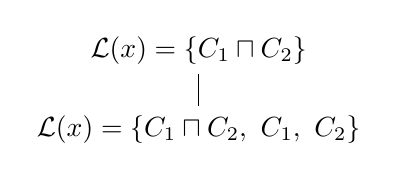
\begin{tikzpicture}[every text node part/.style={align=center},level 1/.style={level distance=1cm, sibling distance=3cm}]
\node [sibling distance=12cm] {$\mathcal{L}(x)=\{C_1\sqcap C_2\}$}
child { node []{$\mathcal{L}(x)=\{C_1\sqcap C_2,~C_1,~C_2\}$}
};
\end{tikzpicture} 
\end{center}
\item[$\sqcup$-rule:] if $C_1\sqcup C_2\in \mathcal{L}(x)$, $x$ is not indirectly blocked and $\{C_1,C_2\} \cap \mathcal{L}(x)\neq \emptyset$, then $ \mathcal{L}(x)\rightarrow 
\mathcal{L}(x)\cup \{C\}~for ~some ~C\in\{C_1,C_2\}$.
\begin{center}
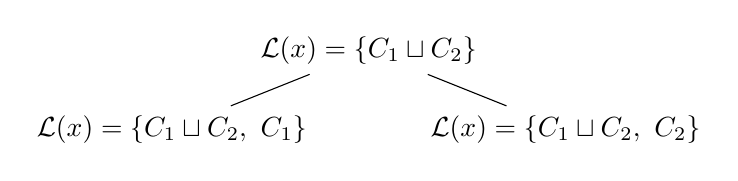
\begin{tikzpicture}[every text node part/.style={align=center},level 1/.style={level distance=1cm, sibling distance=5cm}]
\node [sibling distance=18cm] {$\mathcal{L}(x)=\{C_1\sqcup C_2\}$}
	      child{ node {$\mathcal{L}(x)=\{C_1\sqcup C_2,~C_1\}$}}
	      child{ node {$\mathcal{L}(x)=\{C_1\sqcup C_2,~C_2\}$}};
\end{tikzpicture} 
\end{center}
\item[$\exists$-rule:]  if $\exists r.C\in \mathcal{L}(x)$, $x$ is not blocked and $x$ has no $r$-neighbor $y$ with $C\notin \mathcal{L}(y)$, then create a new node $y$ 
with $\mathcal{E}(\langle x,y\rangle)$ and $\mathcal{L}(y)=\{C\}$.
\begin{center}
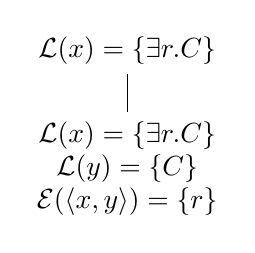
\begin{tikzpicture}[every text node part/.style={align=center},level 1/.style={level distance=1.5cm, sibling distance=3cm}]
\node [sibling distance=12cm] {$\mathcal{L}(x)=\{\exists r.C\}$}
child { node []{$\mathcal{L}(x)=\{\exists r.C\}$ \\ $\mathcal{L}(y)=\{C\}$ \\ $\mathcal{E}(\langle x,y \rangle)=\{r\}$}
};
\end{tikzpicture} 
\end{center}
% \textit{A short discussion:}
% \textit{In the $\exists$-rule, if $\exists r.C\in \mathcal{L}(x)$, a new node is added in two cases : \begin{inparaenum} \item when there exists an edge labeled with $\{r\}$ from $x$ to $y$ and 
% $C \notin  \mathcal{L}(y)$. \item when there does not exist an edge labeled with $\{r\}$ from $x$ to any other nodes. \end{inparaenum}}

\item[$\forall$-rule:] if $\forall r.C\in \mathcal{L}(x)$, $x$ is not indirectly blocked and there exists an $r$-neighbor $y$ of $x$ with $C\notin \mathcal{L}(y)$, then $ \mathcal{L}(y)\rightarrow  \mathcal{L}(y)\cup \{C\}$.
\begin{center}
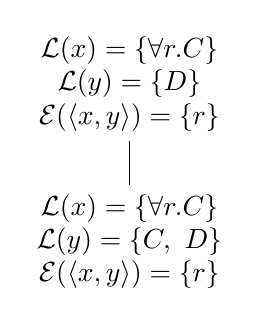
\begin{tikzpicture}[every text node part/.style={align=center},level 1/.style={level distance=2cm, sibling distance=3cm}]
\node [sibling distance=12cm] {$\mathcal{L}(x)=\{\forall r.C\}$\\ $\mathcal{L}(y)=\{D\}$ \\ $\mathcal{E}(\langle x,y \rangle)=\{r\}$}
child { node []{$\mathcal{L}(x)=\{\forall r.C\}$ \\ $\mathcal{L}(y)=\{C, ~D\}$ \\ $\mathcal{E}(\langle x,y \rangle)=\{r\}$}
};
\end{tikzpicture} 
\end{center}
\end{itemize}


The tableau is said to be complete  when there exists a clash in some node $x$ or none of the rules mentioned above can be applied in the tableau. 
For a given concept $D$, $D ~ is ~ satisfiable$ if the tableau is complete without a clash, otherwise   $D ~ is ~ unsatisfiable$.

\begin{mydef}(Clash)
A tableau contains a clash if, for a node $x$ and a concept $C$, $\{C,\neg C\}\subseteq \mathcal{L}(x)$.
\end{mydef}
\begin{center}
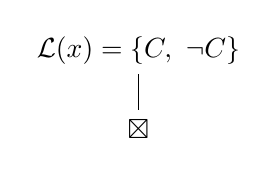
\begin{tikzpicture}[every text node part/.style={align=center},level 1/.style={level distance=1cm, sibling distance=3cm}]
\node [sibling distance=12cm] {$\mathcal{L}(x)=\{C,~\neg C \}$}
child { node []{$\boxtimes$}
};
\end{tikzpicture} 
\end{center}


\section{Qualitative spatial reasoning}\label{sec:qsr}
Qualitative spatial relations such as ``contains", ``left of", ``close to", ``between" can be categorized into three types: topological relations \cite{kuipers1978modeling}, 
directional relative relations and distances \cite{freeman1975modelling}. 
These relations are frequently used at a linguistic level by humans when describing a scene \cite{freksa1991qualitative}.
Even though quantitative information is more precise, human cannot use it as accurate as machine.
Hence through qualitative representation to describe the relation of spatial objects is crucial.
The aim of our study is applying human knowledge to the description of qualitative relationships and the reasoning tasks with spatial objects in a complex scene.
Qualitative spatial reasoning deals with the following questions, among others:
 \begin{itemize}
  \item Can we recognize an object from known objects and their spatial relations?
  \item Which relationships are satisfied between two objects when their relationships are not explicitly described in a given  knowledge base?
  \item Is a recognized spatial arrangement of a scene consistent with the given knowledge of the scene?
 \end{itemize}
 
 The reasoning task can be summarized as follows:
 \begin{enumerate}
  \item Determining whether an object satisfies a spatial configuration, where an object is described by an observation of spatial arrangement and 
  a spatial configuration is defined using expert knowledge. Then the task is considered as a consistency checking  of the observed object with respect to spatial configuration in 
  the knowledge base.
  \item Determining the relationship between two objects from other spatial arrangement. The implicit relation between two objects can be inferred by other known spatial relations
  in a spatial arrangement.
  \item Determining consistency of spatial arrangement in a given configuration of the scene with respect to a specific domain knowledge. This task verifies the consistency
  between the observation and the spatial configuration defined using expert knowledge.
 \end{enumerate}

 In this sections, we discuss different representations of spatial relations and illustrate our formalism to perform spatial reasoning.

\subsection{State of the art}
Spatial relationship is an important factor for image interpretation in brain images due to the similar appearance among brain structures~\cite{Bloch2005fuzzy}.
Chen \textit{et al.} discussed a border range of spatial relation representations~\cite{chen2013survey}. Different spatial calculi are summarized for various aspects of space 
(topology, direction, distance, object shape, etc.). Basic qualitative spatial relations are summarize in Table.\ref{tab:sr}.
\begin{center}
\begin{table}[h]
   \begin{tabular}{| l | c | c |}
    \hline
    Topological relations & Directional relations & Distance relations \\ \hline
    dc (``disconnected from'') & left of & far from \\ 
    eq (``equal with'', ``identical'') & right of & close to \\
    po (``intersect with'', ``partially overlaps'') & above  &   \\
    ec (``external connected with'',``touches'', ``adjacent'') & below &  \\
    tpp (``tangential proper part of'') & in front of &  \\
    tppi (``inversion of tpp'') &  behind  &   \\
    ntpp (``not tangential proper part of'') &   &  \\
    ntppi (``inversion of ntpp'') &  &  \\
    \hline
  \end{tabular}
  \caption{Basic spatial relations}
  \label{tab:sr}  
\end{table}
\end{center}
\subsubsection{Topology}
Topology has been mostly investigated and the most popular representation is based on \textit{Region Connection Calculus} (RCC)~\cite{cohn1997qualitative}.
The collection $\{dc,~eq,~po,~ec,~tpp,~tppi,~ntpp,~ntppi\}$ is a set of disjoint exhaustive topological relations defined as RCC8~\cite{randell1992spatial}.
Between any two objects in topological space, only one of eight relations can be hold.
Therefore, a useful reasoning mechanism of RCC8 based on a composition table is proposed in~\cite{egenhofer1991reasoning} (Table.\ref{tab:comptable}).
Let $A,B,C$ be three objects in topological space, both $A,B$ and $B,C$ are adjacent ($ec$). Then the possible relations between $A,C$ can be found within the table.
This reasoning mechanism allows answer the second and the third questions of qualitative spatial reasoning problems. 
However, the composition table only gives possible relations and many of composition rules give no information like $dc(A,B)$ and $dc(B,C)$ (All the relations are possibly
hold between $A$ and $C$ from the composition table).
Further, the RCC8 representation and composition table were constructed for determining a satisfaction problem 
in a specific arrangement~\cite{wessel2000obstacle,wessel00alcra}.
Unfortunately, the inference within this kind of representation is undecidable~\cite{wessel2000obstacle}. 
Afterwards, Lutz \textit{et al.} exploited qualitative reasoning in concrete domains with constraint satisfaction problems~\cite{lutz2007tableau}.
In the context of brain anatomy, only the inclusion relations are interested~\cite{santos2012region}.
The property of transitivity  is emphasized in this context. 
 \begin{center}
 \begin{table}[H]
 %p{1cm} || p{1cm} | p{1cm} | p{1cm} | p{1cm} | p{1cm} |p{1cm} |p{1cm}| p{1cm}|
    \begin{tabular}{|p{1cm} || p{1.5cm} | p{1.5cm} | p{1.5cm} | p{1.5cm} | p{1.5cm} |p{1.5cm} |p{1.5cm}| p{1.5cm}| }
    \hline
      & $dc$ (B,C) & $\textbf{ec}$ $\textbf{(B,C)}$ & $eq$ (B,C) & $ntpp$  (B,C) & $tpp$ (B,C) &  $ntppi$ (B,C) & $tppi$ (B,C)& $op$ (B,C)\\ \hhline{|=|=|=|=|=|=|=|=|=|}
    $dc$ (A,B) & $dc$ or $ec$ or $eq$ or $ntpp$ or $tpp$ or $ntppi$ or $tppi$ or $op$  & $dc$ or $ec$ or $ntpp$ or $tpp$ or $op$ & $dc$ & $dc$ or $ec$ or $ntpp$ or $tpp$ or $op$ 
		& $dc$ or $ec$ or $ntpp$ or $tpp$ or $op$ & $dc$ &  $dc$ & $dc$ or $ec$ or $ntpp$ or $tpp$ or $op$ \\ \hline 
    $\textbf{ec}$ $\textbf{(A,B)}$ & $dc$ or $ec$ or $eq$ or $ntpp$ or $tpp$ or $ntppi$ or $tppi$ or $op$  & $\textbf{dc~or ec}$ $\textbf{or ntpp}$ $\textbf{or tpp}$ $\textbf{or op}$ & $dc$ 
    & $dc$ or $ec$ or $ntpp$ or $tpp$ or $op$ 	& $dc$ or $ec$ or $ntpp$ or $tpp$ or $op$ & $dc$ &  $dc$ & $dc$ or $ec$ or $ntpp$ or $tpp$ or $op$ \\ \hline 
    $eq$  (A,B) & $dc$ & $ec$ & $eq$ & $ntpp$ & $tpp$ & $ntppi$ & $tppi$ & $op$\\ \hline
    $ntpp$  (A,B)& $dc$ & $dc$ & $ntpp$ & $ntpp$ & $ntpp$ & $dc$ or $ec$ or $eq$ or $ntpp$ or $tpp$ or $ntppi$ or $tppi$ or $op$  & 
		  $dc$ or $ec$ or  $ntpp$ or $tpp$ or $op$& $dc$ or $ec$ or  $ntpp$ or $tpp$ or $op$\\ \hline
    $tpp$  (A,B)& $dc$ & $dc$ or $ec$  & $tpp$ & $ntpp$ & $tpp$ or $ntpp$ & $dc$ or $ec$ or $ntppi$ or $tppi$ or $op$ & $dc$ or $ec$ or $eq$ or $tpp$ or $tppi$ or $op$ &
		   $dc$ or $ec$ or $ntpp$ or $tpp$ or $op$ \\ \hline
    $ntppi$ (A,B)& $dc$ or $ec$ or $ntppi$ or $tppi$ or $op$ & $ntppi$ or $tppi$ or $op$  & $ntppi$ & $eq$ or $ntpp$ or $tpp$ or $tppi$ or $ntppi$ or $op$ &$tppi$ or $ntppi$ or $op$
		  & $ntppi$ &$ntppi$ & $tppi$ or $ntppi$ or $op$ \\ \hline
    $tppi$ (A,B)& $dc$ or $ec$ or $ntppi$ or $tppi$ or $op$  & $ec$ or $ntppi$ or $tppi$ or $op$ & $tppi$ & $ntpp$ or $tpp$ or $op$ & $eq$ or $tpp$ or $tppi$ or $op$ & $ntppi$  &
		  $ntppi$ or $tppi$ & $ntppi$ or $tppi$ or $op$\\ \hline
    $op$ (A,B)& $dc$ or $ec$ or $ntppi$ or $tppi$ or $op$ & $dc$ or $ec$ or $ntppi$ or $tppi$ or $op$ & $op$ & $ntpp$ or $tpp$ or $op$ & $ntpp$ or $tpp$ or $op$ &
		  $dc$ or $ec$ or $ntppi$ or $tppi$ or $op$  & $dc$ or $ec$ or $ntppi$ or $tppi$ or $op$ & $dc$ or $ec$ or $eq$ or $ntpp$ or $tpp$ or $ntppi$ or $tppi$ or $op$\\ \hline
    \end{tabular}
    \caption{The 64 compositions of binary topological relations between objects $A$ and $C$ via the third object $B$. Extracted from~\cite{egenhofer1991reasoning}.}
    \label{tab:comptable}
\end{table}
\end{center} 
\subsubsection{Direction}
Directional relations are seen as primarily important spatial relationships in brain anatomical images~\cite{Bloch2005fuzzy,Hudelot2008fuzzy,nempont2013constraint,fouquier2012sequential}.
As mentioned in~\cite{Bloch2005fuzzy}, a direction is defined by a \textit{target object}, a \textit{reference object} and a \textit{reference system}.
In an 3D space, directional relations are represented by six basic terms (e.g.: right, above, behind, etc.).
In order to compute directional relationships between two objects, many methods such as histograms of angles and morphological approaches are summarized in~\cite{Bloch2005fuzzy}.
Fuzzy representation is employed in these approaches. A fuzzy landscape of a certain direction is computed using morphological dilatation with respect to the reference object.
The satisfaction degree of the direction between the target object and the reference object is evaluated by comparison between the target object and the fuzzy landscape.
In crisp logic, many researches are based on two categories: point based and extend object based (bounding box)~\cite{chen2013survey}.
However, both of two representation ignore the influence of objects forms. The representation is not as accurate to human intuition as fuzzy representation.
% Counter the intuition result by ignoring object form/shape.
% 
% based on mathematical morphology and fuzzy set.
% 
% \cite{santos2012region,cohn1997qualitative,Hudelot2008fuzzy,hudelot2008spatial,
% wessel2000obstacle,wessel00alcra,egenhofer1991reasoning,moratz2003qualitative}
% \subsubsection{Distance}

\subsection{Role Box}
In this section, we give the logical formalism to represent qualitative spatial relationships as roles and  corresponding properties in terms of role axioms within a role box.
% As spatial relations are represented  by roles, a set of role axioms is exploited to model spatial relations.
% In Scenario 1, only topological relations are considered for the spatial reasoning task. 
% A collection (defined as RCC-8: $\{dc, ~eq,~po,~ec,~tpp,~tppi,~ntpp,~ntppi\}$)  is used as a set of disjoint exhaustive topological relations \cite{cohn1997qualitative}.
% In Scenarios 2 and 3, directional relations and distance relations are considered.
% A set of basic spatial relations used in our framework is represented in Table~\ref{tab:sr}. 
% In the following, we denote roles by $u,v,r$, possibly with subscripts. The basic syntax and semantics are described, then role axioms are introduced for spatial reasoning.

\subsubsection{Syntax and semantics of roles}
\begin{mydef}(Role syntax)
 Let $N_R$ be  a set of role names, the inverse roles and the negation of roles are represented by $r^-$ and $\neg r$.
 Complex roles are characterized with $r_1\sqcap r_2$ and $r_1\sqcup r_2$.
 Role axioms are used for modeling properties of roles such as inclusion ($r_1\sqsubseteq r_2$), role composition ($r_1 \circ r_2$).
\end{mydef}
Table \ref{tab:synrole} describes a main syntax and semantics of roles for Description Logics.
\begin{center}
\begin{table}[h]
   \begin{tabular}{| l | c | r |}
    \hline
    Constructor & Syntax & Semantics \\ \hline
    Atomic role & $r$ & $r^\mathcal{I}\subseteq \Delta^\mathcal{I} \times \Delta^\mathcal{I}$ \\
    Inverse role & $r^-$ & $\{\langle x,y\rangle,~x\in \Delta^\mathcal{I},~y\in \Delta^\mathcal{I} | ~(y,x)\in r^\mathcal{I}\}$ \\ 
    Role negation & $\neg r$ & $\Delta^\mathcal{I} \times \Delta^\mathcal{I} \setminus r^\mathcal{I}$ \\
    Role composition & $r_1\circ r_2$ & $\{(x,z), x\in \Delta^\mathcal{I},~z\in \Delta^\mathcal{I}| \exists y\in \Delta^\mathcal{I}, 
\langle x,y\rangle\in r_1^\mathcal{I}~and~(y,z)\in r_2^\mathcal{I}\}$  \\
    Role conjunction & $r_1\sqcap r_2$ & $r_1^\mathcal{I} \cap r_2^\mathcal{I}$ \\
    Role disjunction & $r_1\sqcup r_2$ & $r_1^\mathcal{I} \cup r_2^\mathcal{I}$ \\
    Role inclusion & $r_1\sqsubseteq r_2$ &  $r_1^\mathcal{I} \subseteq r_2^\mathcal{I}$\\
    Role equivalence & $r_1\equiv r_2$ & $r_1^\mathcal{I} = r_2^\mathcal{I}$\\
    \hline
  \end{tabular}
  \caption{Basic spatial relations}
  \label{tab:synrole}  
\end{table}
\end{center}

\begin{mydef}(Role inclusion axiom) 
 A role inclusion axiom is defined in the form:
 $$r\sqsubseteq s,$$
 where $r$ and $s$ are basic roles in $N_R$ or complex roles built with role constructors. A role equivalence $r\equiv s$ can be rewritten in the form $r\sqsubseteq s$ and $s\sqsubseteq r$.
\end{mydef}
\begin{mydef}(RBox)
A role box, denoted by RBox, is a finite set
% \footnote{ Jamal has noted ``$\mathfrak{C}$ is infinite''. But I do not understand very well. A RBox is independent of concept expressions, which
% represents a set of properties of roles.}
of axioms for $N_R$  based on a set of roles $\mathbf{R}=N_R\cup\{r^-| r\in N_R\}$, where $r^-$  represents the inversion of role $r$.
Based on role inclusions and role equivalences, role axioms characterize role properties such that:
\begin{itemize}
 \item role composition: $u\circ v \sqsubseteq r_1\sqcup \cdots\sqcup r_n$ with $n\geqslant 1$, which is interpreted as 
 $(u\circ v)^\mathcal{I} \subseteq r_1^\mathcal{I} \cup \cdots \cup r_n^\mathcal{I}$. If there exists three interpretation elements $x,y,z\in \Delta^\mathcal{I}$, 
 $\langle x,y \rangle \in u^\mathcal{I}$ and $\langle y,z \rangle \in v^\mathcal{I}$ implies  $\langle x,z \rangle \in r_1^\mathcal{I} \cup \cdots \cup r_n^\mathcal{I}$. 
 \item transitive role: $r\circ r \sqsubseteq r$, which is interpreted as $(r\circ r)^\mathcal{I} \subseteq r^\mathcal{I}$. If there exists three interpretation elements
 $x,y,z\in \Delta^\mathcal{I}$, $\langle x,y \rangle \in r^\mathcal{I}$ and $\langle y,z \rangle \in r^\mathcal{I}$ implies  $\langle x,z \rangle \in r^\mathcal{I}$.
 \item inverse roles: $u \equiv v^-$, which is interpreted as $u^\mathcal{I} = v^{-\mathcal{I}}$. There exists two interpretation elements  $x,y\in \Delta^\mathcal{I}$,
 then $\langle x,y \rangle \in u^\mathcal{I}$ iff $\langle y,x \rangle \in v^\mathcal{I}$.
 \item symmetric role: $r \equiv r^-$, which is interpreted as $r^\mathcal{I} = r^{-\mathcal{I}}$. There exists two interpretation elements  $x,y\in \Delta^\mathcal{I}$,
 then $\langle x,y \rangle \in r^\mathcal{I}$ iff $\langle y,x \rangle \in r^\mathcal{I}$.
 \item disjoint roles: $u\sqsubseteq \neg v$. which is interpreted as $u^\mathcal{I} \subseteq \Delta^\mathcal{I} \setminus v^\mathcal{I}$ or $u^\mathcal{I}\cap v^\mathcal{I}=\emptyset$. 
 There exists two interpretation elements  $x,y\in \Delta^\mathcal{I}$, 
$\langle x,y \rangle \in u^\mathcal{I}$ implies $\langle x,y \rangle \notin v^\mathcal{I}$.
\end{itemize}
\end{mydef}
The knowledge base used for spatial reasoning in our framework is built with three blocks: terminologies (TBox), role axioms (RBox) and assertions (ABox)
($\mathcal{K}=\{\mathcal{T},\mathcal{R},\mathcal{A}\}$).

To ensure the termination of tableau construction, a mechanism for detecting cyclic expansions called \textit{blocking} is used.
To define \textit{blocking}, we first introduce the term \textit{$r$-neighbor}.
\begin{mydef}($r$-neighbor)
In the tableau, an edge $\langle x,y \rangle$ labeled with role $r$ relates two nodes $x$ and $y$,
$y$ is called a successor of $x$ and $x$ is called  a predecessor of $y$. An ancestor is the transitive closure of predecessor,
where the transitive closure refers to an indirect reachability relation constructed from a set of direct edges.
A node $y$ is a $r$-neighbor of a node $x$ if
\begin{itemize}
\item $x$ is a predecessor of $y$ and $\mathcal{E}(\langle x,y\rangle)=\{r\}$.
% \item $y$ is a predecessor of $x$ and $\mathcal{E}(\langle y,x\rangle)=r^-$.
\end{itemize}
\end{mydef}


\begin{mydef}(Blocking)

\begin{itemize}
\item A node $x$ is directly blocked, which indicates that it has a unique ancestor $y$ such that $\mathcal{L}(y)=\mathcal{L}(x)$.
\item  Otherwise, it is indirectly blocked if its predecessor $y$ is blocked by another ancestor $u$.
\end{itemize}
A node $x$ is blocked if for some ancestor $y$, $y$ is blocked or $\mathcal{L}(y)=\mathcal{L}(x)$. 
\end{mydef}

\subsection{From image to symbolic representation}
The transformation of representation from low-level numerical data to symbolic level is first phase of the framework.
Concretely, objects and contextual information are extracted and represented within terminologies using an ABox.

\subsection{Spatial reasoning using tableaux method}

\section{Abductive reasoning}\label{sec:abd}
% This part includes a short introduction of what an abductive reasoning is. Then why this is suitable for image interpretation task.
% In the end two elements of abductive is important to resolved in this thesis.

Abductive reasoning is a backward-chaining inference, concerned generating hypotheses and finding the ``best'' explanation on the basis of surprising observation.
Unlike the inference operation of standard reasoning presented in Section.\ref{sec:pre}, abductive reasoning is a non-monotonic reasoning.
New knowledge should be added in order to positively entail the observation.
Image interpretation for a diagnostic problem fits abductive reasoning  mechanism.
When facing an pathological brain imaging, an expert has to resort to his knowledge of pathological anatomy, in order to give  an explanation for observed image. 
In this section, we will introduce how abductive is applied in image interpretation task from two aspects (generation and selection).

% Useful words:
%    Inference operation.
% abduction is not a simple exploitation in knowledge base, but a task of adding new knowledge to acquire satisfied results. 
\subsection{State of the art of abductive reasoning}
Abductive reasoning is first proposed by Charles S. Peirce in philosophy.
Afterwards, abductive is developed in artificial intelligence and cognitive science.
Aliseda~\cite{aliseda1997seeking} gave a general overview of abduction in propositional logic and proposed tableaux methods for abduction.
Further, in the context of Description Logics, four types of abduction problems  are described by Elisenbroich~\cite{elsenbroich2006case}.
Let $\mathcal{L}$ be a DL, $\mathcal{K}=\{\mathcal{T},\mathcal{A}\}$ be a knowledge base in $\mathcal{L}$, $C,D$ two concepts in $\mathcal{L}$ and suppose that they are satisfiable
with respect to  $\mathcal{K}$.
The logical formalisms of abduction in DLs are represented as follows:
\begin{itemize}
 \item Concept abduction: given an observation concept $O$, a hypothesis is a concept $H$ such that $\mathcal{K}\vDash H \sqsubseteq O$.
 \item TBox abduction: 
 \item ABox abduction: let $S_a$ be a set of assertions as observation, a hypothesis is a set of $S_b$ of ABox assertion such that $\mathcal{K} \cup S_b\vDash \phi(a)$.
 \item Knowledge base abduction:
\end{itemize}


\cite{neumann2008scene} use DL-safe rules( expressive but preserve decidability).
\cite{shanahan2005perception} multimedia interpretation as abduction.
\cite{colucci2004uniform,di2009tableaux} adapted tableaux methods in Description Logics formalisms.
\cite{bienvenu08complexity} discussed a set of basic minimality criteria for abductive reasoning.
\cite{aliseda1997seeking,elsenbroich2006case,colucci2004uniform,di2009tableaux,klarman2011abox,halland2014tbox,gries2010probabilistic,du2011towards,du2014tractable,bienvenu08complexity}
\subsection{Abductive reasoning for image interpretation}
In the context of image interpretation,
\subsection{Minimality criteria}
\textit{Abduction as Inference to the Best Explanation.}
filter inconsistent and redundant ones

\section{Perspectives}\label{sec:persp}
Several directions will be presented in this section:
\begin{itemize}
 \item concrete domain with fuzzy logic.
 \item how to generate potential hypotheses.
 \item how to select the ``best'' explication with an appropriate minimality criterion.
 \item perspective of publications.
\end{itemize}

\section{Activities}
\begin{itemize}
 \item project LOGIMA
 \item seminars
 \item doctoral formation
\end{itemize}

% \nocite{*}
\bibliographystyle{plain}
\bibliography{mi_ref}
\end{document}


% \section{Tableaux method}
% First of all, we recall the expansion rules of the tableau method in $\mathcal{ALCI_{R_+}}$.
% 
% \begin{mydef}($\mathcal{ALCHI_{R+}}$ tableau)
% Let $D$ be an $\mathcal{ALC}$ concept in NNF and let $R_D$ be the set of roles in $\mathcal{ALC}$, a tableau $T$ for $D$ is defined as a triple $(\mathbf{S},\mathcal{L}, \mathcal{E})$, 
% where $\mathbf{S}$ is a set of interpretation elements; 
% $\mathcal{L}$ relates each interpretation element to a set of concepts occurring in $D$ (from $\mathbf{S}$ to $\mathcal{P}(\mathfrak{C}$)); 
% $\mathcal{E}$ relates each pair of interpretation elements to a set of roles in $R_D$  (from $\mathbf{S}\times\mathbf{S}$ to $\mathcal{P}(R_D)$). 
% 
% The decision procedure to check the satisfiability of a given concept $D$ is based on constructing a model using the tableau method. 
% Let $x$ and $y$ be two interpretation elements in $\mathbf{S}$ ($x,~y\in \mathbf{S}$), $C,E$ be two concepts occurring in $D$ and $r\in R_D$.
% The model is constructed as a tree structure where each node corresponds to an element of interpretation $x\in \Delta^\mathcal{I}$.
% The node is labeled with a set of concepts $\mathcal{L}(x)$.
% The edge between the nodes $x$ and $y$ is labeled with corresponding roles $r\in\mathcal{E}(\langle x,y \rangle)$.
% The following conditions hold:
% \begin{itemize}
% \item if $C\in \mathcal{L}(x)$, then $\neg C\notin\mathcal{L}(x)$.
% \item if $C\sqcap E\in \mathcal{L}(x)$, then $ C\in\mathcal{L}(x)$ and $ E\in\mathcal{L}(x)$.
% \item if $C\sqcup E\in \mathcal{L}(x)$, then $ C\in\mathcal{L}(x)$ or $ E\in\mathcal{L}(x)$.
% \item if $\exists r.C\in \mathcal{L}(x)$, then there exists some $y\in \mathbf{S}$  such that $r \in \mathcal{E}(\langle x,y\rangle)$ and $C\in\mathcal{L}(y)$.
% \item if $\forall r.C\in \mathcal{L}(x)$, then for all  existing $y \in \mathbf{S}$ such that $r \in \mathcal{E}(\langle x,y\rangle)$, $C\in\mathcal{L}(y)$.
% \item if $\forall r.C\in \mathcal{L}(x)$, $r \in \mathcal{E}(\langle x,y\rangle)$ and $r$ is a transitive role, then $\forall r.C\in \mathcal{L}(y)$.
% \item if $\forall r.C\in \mathcal{L}(x)$, $v \in \mathcal{E}(\langle x,y\rangle)$, $v\sqsubseteq r$ (or $v^-\sqsubseteq r^-$) and $v$ is a transitive role, then $\forall v.C\in \mathcal{L}(y)$.
% \item $r \in \mathcal{E}(\langle x,y\rangle)$ iff  $ r^-\in \mathcal{E}(\langle y,x\rangle)$.
% \item $ r\in \mathcal{E}(\langle x,y\rangle)$ and $r\sqsubseteq v$ (or $r^-\sqsubseteq v^-$) then  $v \in \mathcal{E}(\langle x,y\rangle)$.
% \end{itemize}
% \end{mydef}
% \section{Example}
%  The complete knowledge base is given as follows:
% \begin{align*}
%  TBox=\{ Hemisphere &\sqsubseteq \exists isPartOf. Brain\\
% 	 BrainStructure &\sqsubseteq \exists isPartOf. Brain\\
% 	 BrainDisease &\sqsubseteq \exists isPartOf. Brain \sqcap \neg BrainStructure\\
% 	 Tumor  &\sqsubseteq BrainDisease\\
% 	 LVl &\sqsubseteq BrainStructure \sqcap \exists (rightOf \sqcap closeTo). CNl\\
% 	 LVr &\sqsubseteq BrainStructure \sqcap \exists (leftOf \sqcap closeTo). CNr\\
% 	 CNl &\sqsubseteq BrainStructure\\
% 	 CNr &\sqsubseteq BrainStructure\}
% % 	 WMl &\sqsubseteq BrainStructure\\
% % 	 WMr &\sqsubseteq BrainStructure\\
% % 	 PUl &\sqsubseteq BrainStructure\\
% % 	 PUr &\sqsubseteq BrainStructure\\
% % 	 THl &\sqsubseteq BrainStructure\\
% % 	 THr &\sqsubseteq BrainStructure\}
% \end{align*}
% The role axioms are described as:
% \begin{align*}
%  RBox=\{ rightOf &\equiv leftOf^-\\
%          above &\equiv below^- \\
% 	 closeTo &\equiv closeTo^- \\
% 	 farFrom &\equiv farFrom^- \\
% 	 isPartOf \circ isPartOf &\sqsubseteq isPartOf \\
% 	 hasPart \circ hasPart &\sqsubseteq hasPart\\
% 	 isPartOf &\equiv hasPart^-\}
% \end{align*}
% 
% % The ABox is used for describing the observation in the image.
% % The spatial configuration describes the relationships between different structures.
% The ABox represents the observation of recognized structures and the relationships with others.
% For example, a region is recognized as the left caudate nucleus (CNl), denoted by $a$.
% The region of brain is denoted by $c$. An unknown region is segmented and their relationships are computed.  
% Such an observation can be represented as
% % \footnote{At first, I assume to use a threshold to convert quantification measures to qualitative representations. However, the threshold 
% % is hard to choose. If we use a fuzzy ABox, only the spatial relations are assigned with a satisfaction degree. However, I have not read the reference about reasoning service on fuzzy Description Logics yet.}:
% \begin{align*}
%  ABox=\{ a&: CNl \\
% 	 b&: unknown \\
% 	 c&: Brain \\
% 	 \langle a,b\rangle &: leftOf, closeTo \\
% 	 \langle b,c\rangle &: isPartOf\}
% \end{align*}
% 
% % In an image understanding application, we reason about a description which explains a given image in a certain domain.
% In this example, the ABox describes an observation of a given scene and the objective is to find a reasonable description of  the unknown object $b$.
% % This type of reasoning can be treated as an abductive reasoning.
% A possible hypothesized description is $LVl\sqcap \exists isPartOf.Hemisphere$.
% The hypothesis can be verified by a concept subsumption checking: $\mathcal{K} \vDash H\sqsubseteq O$, where $H$ is the explained concept for the observation $O$.
% To check subsumption of two concepts $H$ and $O$, $\mathcal{K} \vDash H\sqcap \neg O \sqsubseteq \bot$ is required to prove that $H\sqcap \neg O$ is unsatisfiable.
% 
% In this example, $O\equiv \exists (leftOf^-\sqcap closeTo^-).CNl\sqcap \exists isPartOf.Brain$ and $H\equiv LVl\sqcap \exists isPartOf.Hemisphere$.
% Let $x$ be the interpretation element of the concept $H\sqcap \neg O$. 
% 
% The tableau is initialized with $\mathcal{L}(x)=\{ LVl\sqcap \exists isPartOf.Hemisphere\sqcap \forall (leftOf^-\sqcap closeTo^-).CNl\sqcup \forall isPartOf.\neg Brain\}$.
% The $\sqcap$, $\sqcup$ rules are applied and we obtain:
% \begin{center}
% \begin{tikzpicture}[every text node part/.style={align=center},level 1/.style={level distance=1.5cm, sibling distance=9cm}]
% \node [sibling distance=18cm] {$\mathcal{L}(x)=\{ LVl\sqcap \exists isPartOf.Hemisphere\sqcap \forall (leftOf^-\sqcap closeTo^-).CNl\sqcup \forall isPartOf.\neg Brain\}$}
% 	      child{ node {$\mathcal{L}(x)=\{ LVl,~\exists isPartOf.Hemisphere,$\\$~\forall (leftOf^-\sqcap closeTo^-).\neg CNl\}$}}
% 	      child{ node {$\mathcal{L}(x)=\{ LVl,~\exists isPartOf.Hemisphere,$\\$~\forall isPartOf.\neg Brain\}$}};
% \end{tikzpicture} 
% \end{center}
% 
% To integrate terminological knowledge, axioms in the form $C\sqsubseteq D$ in TBox can be internalized into single concepts ($\neg C\sqcup D$) and added to $\mathcal{L}(x)$. Here, for the sake of simplicity 
% of demonstration, we only add the internalization of the axiom $LVl \sqsubseteq BrainStructure \sqcap  \exists (rightOf \sqcap closeTo). CNl$ for the first branch.
% \begin{center}
% \begin{tikzpicture}[every text node part/.style={align=center},level 1/.style={level distance=1.5cm, sibling distance=9cm}]
% \node [sibling distance=18cm] {$\mathcal{L}(x)=\{ LVl\sqcap \exists isPartOf.Hemisphere\sqcap \forall (leftOf^-\sqcap closeTo^-).CNl\sqcup \forall isPartOf.\neg Brain\}$}
% 	      child{ node {$\mathcal{L}(x)=\{ LVl,~\exists isPartOf.Hemisphere,$\\$~\forall (leftOf^-\sqcap closeTo^-).\neg CNl,$\\$\neg LVl \sqcup BrainStructure \sqcap \exists (rightOf \sqcap closeTo).CNl\}$}}
% 	      child{ node {$\mathcal{L}(x)=\{ LVl,~\exists isPartOf.Hemisphere,$\\$~\forall isPartOf.\neg Brain\}$}};
% \end{tikzpicture}  
% \end{center}
% 
% We then apply $\sqcup$ and $\sqcap$ rules again on the first branch:
% \begin{center}
% \begin{tikzpicture}[every text node part/.style={align=center},level 1/.style={level distance=1.5cm, sibling distance=9cm}, level 2/.style={level distance=2cm, sibling distance=6cm}]
% \node [sibling distance=18cm] {$\mathcal{L}(x)=\{ LVl\sqcap \exists isPartOf.Hemisphere\sqcap \forall (leftOf^-\sqcap closeTo^-).\neg CNl\sqcup \forall isPartOf.\neg Brain\}$}
% 	      child{ node {$\mathcal{L}(x)=\{ LVl,~\exists isPartOf.Hemisphere,$\\$~\forall (leftOf^-\sqcap closeTo^-).\neg CNl,$\\$\neg LVl \sqcup BrainStructure \sqcap \exists (rightOf \sqcap closeTo).CNl\}$}
% 	      		    child{ node {$\mathcal{L}(x)=\{ LVl,~\exists isPartOf.Hemisphere,$\\$~\forall (leftOf^-\sqcap closeTo^-).\neg CNl,$\\$\neg LVl\}$}
% 				  child{ node{$\boxtimes$}}}
% 		            child{ node {$\mathcal{L}(x)=\{ LVl,~\exists isPartOf.Hemisphere,$\\$~\forall (leftOf^-\sqcap closeTo^-). \neg CNl,$\\$BrainStructure,$\\$\exists (rightOf \sqcap closeTo).CNl$}}}
% 	      child{ node {$\mathcal{L}(x)=\{ LVl,~\exists isPartOf.Hemisphere,$\\$~\forall isPartOf.\neg Brain\}$}};
% \end{tikzpicture}  
% \end{center}
% 
% A clash ($LVl,~\neg LVl$) is detected in the first part of the first branch (closed). We then apply $\exists$ on the second part:
% \begin{center}
% \begin{tikzpicture}[every text node part/.style={align=center},level 1/.style={level distance=1.5cm, sibling distance=9cm}, level 2/.style={level distance=2cm, sibling distance=6cm},
% level 3/.style={level distance=2.5cm, sibling distance=6cm}]
% \node [sibling distance=18cm] {$\mathcal{L}(x)=\{ LVl\sqcap \exists isPartOf.Hemisphere\sqcap \forall (leftOf^-\sqcap closeTo^-).\neg CNl\sqcup \forall isPartOf.\neg Brain\}$}
% 	      child{ node {$\mathcal{L}(x)=\{ LVl,~\exists isPartOf.Hemisphere,$\\$~\forall (leftOf^-\sqcap closeTo^-).\neg CNl,$\\$\neg LVl \sqcup BrainStructure \sqcap \exists (rightOf \sqcap closeTo).CNl\}$}
% 	      		    child{ node {$\mathcal{L}(x)=\{ LVl,~\exists isPartOf.Hemisphere,$\\$~\forall (leftOf^-\sqcap closeTo^-).\neg CNl,$\\$\neg LVl\}$}
% 				  child{ node{$\boxtimes$}}}
% 		            child{ node {$\mathcal{L}(x)=\{ LVl,~\exists isPartOf.Hemisphere,$\\$~\forall (leftOf^-\sqcap closeTo^-).\neg CNl,$\\$BrainStructure,$\\$\exists (rightOf \sqcap closeTo).CNl$}
% 				  child{ node {$\mathcal{L}(x)=\{ LVl,~\exists isPartOf.Hemisphere,$\\
% 				  $~\forall (leftOf^-\sqcap closeTo^-).\neg CNl,$\\$BrainStructure,$\\$\exists (rightOf \sqcap closeTo).CNl$\\
% 				  $\mathcal{L}(y)=\{CNl\}$\\
% 				  $\mathcal{E}(\langle x,y \rangle)=\{rightOf,closeTo\}$}}}}
% 	      child{ node {$\mathcal{L}(x)=\{ LVl,~\exists isPartOf.Hemisphere,$\\$~\forall isPartOf.\neg Brain\}$}};
% \end{tikzpicture}  
% \end{center}
% 
% Because of inverse role axioms in RBox, we can add inverse roles in $\mathcal{E}(\langle x,y \rangle)$ and apply  $\forall$ rule on the second part:
% \begin{center}
% \begin{tikzpicture}[every text node part/.style={align=center},level 1/.style={level distance=1.5cm, sibling distance=9cm}, level 2/.style={level distance=2cm, sibling distance=6cm},
% level 3/.style={level distance=2.5cm, sibling distance=6cm}]
% \node [sibling distance=18cm] {$\mathcal{L}(x)=\{ LVl\sqcap \exists isPartOf.Hemisphere\sqcap \forall (leftOf^-\sqcap closeTo^-).\neg CNl\sqcup \forall isPartOf.\neg Brain\}$}
% 	      child{ node {$\mathcal{L}(x)=\{ LVl,~\exists isPartOf.Hemisphere,$\\$~\forall (leftOf^-\sqcap closeTo^-).\neg CNl,$\\$\neg LVl \sqcup BrainStructure \sqcap \exists (rightOf \sqcap closeTo).CNl\}$}
% 	      		    child{ node {$\mathcal{L}(x)=\{ LVl,~\exists isPartOf.Hemisphere,$\\$~\forall (leftOf^-\sqcap closeTo^-).\neg CNl,$\\$\neg LVl\}$}
% 				  child{ node{$\boxtimes$}}}
% 		            child{ node {$\mathcal{L}(x)=\{ LVl,~\exists isPartOf.Hemisphere,$\\$~\forall (leftOf^-\sqcap closeTo^-).\neg CNl,$\\$BrainStructure,$\\$\exists (rightOf \sqcap closeTo).CNl$}
% 				  child{ node {$\mathcal{L}(x)=\{ LVl,~\exists isPartOf.Hemisphere,$\\
% 				  $~\forall (leftOf^-\sqcap closeTo^-).\neg CNl,$\\$BrainStructure,$\\$\exists (rightOf \sqcap closeTo).CNl$\\
% 				  $\mathcal{L}(y)=\{CNl,~\neg CNl\}$\\
% 				  $\mathcal{E}(\langle x,y \rangle)=\{rightOf,closeTo,leftOf^-,closeTo^-\}$\\
% 				  $\mathcal{L}(y,x)=\{rightOf^-,closeTo^-,leftOf,closeTo\}$}
% 				  child{ node{$\boxtimes$}}}}}
% 	      child{ node {$\mathcal{L}(x)=\{ LVl,~\exists isPartOf.Hemisphere,$\\$~\forall isPartOf.\neg Brain\}$}};
% \end{tikzpicture}  
% \end{center}
% 
% The first branch of the tableau is closed because of the clash of $CNl$ and $\neg CNl$ in the second part. We then explore the second branch. At first we apply the $\exists$ rule and then $\forall$ rule:
% \begin{center}
% \begin{tikzpicture}[every text node part/.style={align=center},level 1/.style={level distance=1.5cm, sibling distance=9cm}, level 2/.style={level distance=2cm, sibling distance=6cm},
% level 3/.style={level distance=2.5cm, sibling distance=6cm}]
% \node [sibling distance=18cm] {$\mathcal{L}(x)=\{ LVl\sqcap \exists isPartOf.Hemisphere\sqcap \forall (leftOf^-\sqcap closeTo^-).\neg CNl\sqcup \forall isPartOf.\neg Brain\}$}
% 	      child{ node {$\mathcal{L}(x)=\{ LVl,~\exists isPartOf.Hemisphere,$\\$~\forall (leftOf^-\sqcap closeTo^-).\neg CNl,$\\$\neg LVl \sqcup BrainStructure \sqcap \exists (rightOf \sqcap closeTo).CNl\}$}
% 				  child{ node{$\boxtimes$}}}
% 	      child{ node {$\mathcal{L}(x)=\{ LVl,~\exists isPartOf.Hemisphere,$\\$~\forall isPartOf.\neg Brain\}$}
% 		     child{ node{$\mathcal{L}(x)=\{ LVl,~\exists isPartOf.Hemisphere,$\\$~\forall isPartOf.\neg Brain\}$\\
% 				  $\mathcal{L}(y)=\{ Hemisphere, \neg Brain, \forall isPartOf. \neg Brain\}$\\
% 				  $\mathcal{E}(\langle x,y \rangle)=\{isPartOf\}$}}};
% \end{tikzpicture}  
% \end{center}
% 
% The axiom $Hemisphere \sqsubseteq \exists isPartOf.Brain$ is internalized and added into $\mathcal{L}(y)$. Then we continue to extend the second branch with expansion rules:
% \begin{center}
% \begin{tikzpicture}[every text node part/.style={align=center},level 1/.style={level distance=1.5cm, sibling distance=7cm}, level 2/.style={level distance=2cm, sibling distance=6cm},
% level 3/.style={level distance=3cm, sibling distance=8cm}]
% \node [sibling distance=18cm] {$\mathcal{L}(x)=\{ LVl\sqcap \exists isPartOf.Hemisphere\sqcap \forall (leftOf^-\sqcap closeTo^-).\neg CNl\sqcup \forall isPartOf.\neg Brain\}$}
% 	      child{ node {$\mathcal{L}(x)=\{ LVl,~\exists isPartOf.Hemisphere,$\\$~\forall (leftOf^-\sqcap closeTo^-).\neg CNl,$\\$\neg LVl \sqcup BrainStructure \sqcap \exists (rightOf \sqcap closeTo).CNl\}$}
% 				  child{ node{$\boxtimes$}}}
% 	      child{ node {$\mathcal{L}(x)=\{ LVl,~\exists isPartOf.Hemisphere,$\\$~\forall isPartOf.\neg Brain\}$}
% 		     child{ node{$\mathcal{L}(x)=\{ LVl,~\exists isPartOf.Hemisphere,$\\$~\forall isPartOf.\neg Brain\}$\\
% 				  $\mathcal{L}(y)=\{ Hemisphere, \neg Brain, \forall isPartOf. \neg Brain$\\
% 				  $\neg Hemisphere \sqcup \exists isPartOf.Brain\}$\\
% 				  $\mathcal{E}(\langle x,y \rangle)=\{isPartOf\}$}
% 				  child{ node{$\mathcal{L}(x)=\{ LVl,~\exists isPartOf.Hemisphere,$\\$~\forall isPartOf.\neg Brain\}$\\
% 					      $\mathcal{L}(y)=\{ Hemisphere, \neg Brain, \forall isPartOf. \neg Brain,$\\
% 					      $\neg Hemisphere\}$\\
% 					      $\mathcal{E}(\langle x,y \rangle)=\{isPartOf\}$ }
% 					      child{ node{$\boxtimes$}}}
% 				  child{ node{$\mathcal{L}(x)=\{ LVl,~\exists isPartOf.Hemisphere,$\\$~\forall isPartOf.\neg Brain\}$\\
% 					      $\mathcal{L}(y)=\{ Hemisphere, \neg Brain, \forall isPartOf. \neg Brain$,\\
% 					      $ \exists isPartOf.Brain\}$\\
% 					      $\mathcal{E}(\langle x,y \rangle)=\{isPartOf\}$ }
% 					child{ node{$\mathcal{L}(x)=\{ LVl,~\exists isPartOf.Hemisphere,$\\$~\forall isPartOf.\neg Brain\}$\\
% 						    $\mathcal{L}(y)=\{ Hemisphere, \neg Brain, \forall isPartOf. \neg Brain$,\\
% 						    $ \exists isPartOf.Brain\}$\\
% 						    $\mathcal{E}(\langle x,y \rangle)=\{isPartOf\}$\\
% 						    $\mathcal{L}(z)=\{Brain,\neg Brain,\forall isPartOf.\neg Brain\}$\\
% 						    $\mathcal{E}(\langle y,z\rangle)=\{isPartOf\}$}
% 						    child{ node{$\boxtimes$}}}}}};
% \end{tikzpicture}  
% \end{center}
% 
% In both two parts of the second branch, we get clashes ($Hemisphere$ and $\neg Hemisphere$ in $\mathcal{L}(y)$ for the first part, $Brain$ and $\neg Brain$ in $\mathcal{L}(z)$ for the second part).
% This implies we can not find a model for the concept $H\sqcap \neg O$. Therefore, it is unsatisfiable and we can conclude that $K\vDash H\sqsubseteq O$ and $LVl\sqcap \exists isPartOf.Hemisphere$ is a potential
% explication of the observation.

